\documentclass[paper=a4wide, fontsize=12pt]{scrartcl}	 % A4 paper and 11pt font size
\usepackage[svgnames]{xcolor} % Using colors
\usepackage{background} % To include background images
\usepackage{fancyhdr} % Needed to define custom headers/footers
\usepackage[a4paper, left=20mm, right=20mm, top=20mm, bottom=2.5cm, footskip=1.2cm]{geometry}  % Changing size of document
%\usepackage[square, numbers, comma, sort&compress]{natbib} % Use the natbib reference package - read up on this to edit the reference style; if you want text (e.g. Smith et al., 2012) for the in-text references (instead of numbers), remove 'numbers'


\usepackage{braket}
\usepackage[utf8]{vietnam}
\usepackage{hyperref}
\usepackage{float}
\usepackage{subcaption}

%%%%%% Setting up the style

\setlength\parindent{0pt} % Gets rid of all indentation
\backgroundsetup{contents={\includegraphics[width=\textwidth]{banner_uit.png}},scale=0.5,placement=top,opacity=0.4} %  OIST Logo

\pagestyle{fancy} % Enables the custom headers/footers

\lhead{} \rhead{} % Headers - all  empty

\title{\vspace{-1.8cm}  \color{DarkRed}  Đồ án môn học IE221.N21.CNCL}
\subtitle{SwiftSend - Global File Sharing-Transfering % Title of the rotation project
\vspace{-2cm} }
\date{} % No date

\lfoot{\color{Grey} Nguyễn Hoàng Tân}  % Write your name here
\rfoot{\color{Grey} KHCL2021.1}
\cfoot{\color{Grey} \thepage}

\renewcommand{\headrulewidth}{0.0pt} % No header rule
\renewcommand{\footrulewidth}{0.4pt} % Thin footer rule

%%%%%% Starting the document

\begin{document}

\maketitle % Print the title
\thispagestyle{fancy} % Enabling the custom headers/footers for the first page


% In the following lines, add the relevant information
\vspace{-0.5cm} \textbf{Sinh viên thực hiện: Nguyễn Hoàng Tân}

\textbf{MSSV: 21521413}

\textbf{Ngày nộp báo cáo: 31/05/2023}

\textbf{Giảng viên: Nguyễn Thanh Sơn}

\textbf{Source code: \href{https://github.com/Dev-Aligator/SwiftSend-Web}{Repo:SwiftSend}}





\vspace{0.5cm}

\section{Giới thiệu đồ án}

SwiftSend là một nền tảng chia sẻ tập tin nhanh chóng và dễ sử dụng, mang lại trải nghiệm tuyệt vời cho người dùng khi có thể dễ dàng truy cập thông qua trình duyệt web. Dự án được phát triển bằng Django, một framework phát triển ứng dụng web mạnh mẽ và linh hoạt dựa trên ngôn ngữ lập trình Python. \\

Với SwiftSend, người dùng có thể chia sẻ và nhận các tập tin lớn một cách nhanh chóng và dễ dàng không chỉ giới hạn trên mạng nội bộ mà còn trên toàn cầu. Giao diện người dùng đơn giản và thân thiện giúp mọi người dễ dàng làm quen và sử dụng ứng dụng này một cách hiệu quả. \\

Dự án mang đến nhiều tính năng thú vị như tạm dừng và tiếp tục quá trình chia sẻ, giám sát trạng thái chuyển giao tập tin trực tiếp và xử lý lỗi một cách tin cậy, đảm bảo việc chuyển giao tập tin luôn mượt mà và bảo mật. \\

Ngoài ra, SwiftSend còn cho phép người dùng tạo phòng riêng tư để chia sẻ tập tin một cách an toàn và tùy chỉnh hồ sơ cá nhân để tạo điểm nhấn riêng biệt. Người dùng có thể chia sẻ tập tin với một lượng lớn người dùng, từ một nhóm nhỏ đến cả một cộng đồng lớn. \\

Dự án mang lại sự tự do và linh hoạt cho người dùng khi kết nối, cộng tác và trao đổi tập tin trong một môi trường an toàn và tùy chỉnh. \\

Phần tiếp theo của báo cáo này trình bày chi tiết về các tính năng của SwiftSend và cách nó mang lại lợi ích cho người dùng.

\section{Tóm tắt quá trình thực hiện}
Phần này ghi lại quá trình thực hiện đồ án trong 3 tuần qua
\subsection{Tuần đầu tiên}
Trong tuần đầu tiên, tập trung vào thiết lập cơ bản của ứng dụng. Cho phép người dùng tạo tài khoản và đăng nhập vào hệ thống. Ngoài ra, xây dựng trang chủ, trang quản trị, trang hồ sơ cá nhân và Chat bot để mang lại trải nghiệm toàn diện cho người dùng. Mình cũng đã triển khai chức năng chuyển đổi giao diện (Theme switcher) để người dùng có thể tùy chỉnh giao diện theo sở thích của mình.
\subsection{Tuần thứ 2}
Trong tuần thứ hai, mình triển khai chức năng tải tập tin thông qua các \textbf{"Department"} định sẵn một cách công khai . Người dùng có thể tải lên tập tin và chia sẻ chúng với những người khác trong hệ thống. Đồng thời, thực hiện chức năng "Phê duyệt" (Accept) để mỗi tập tin cần được phê duyệt bởi quản trị viên trước khi có thể truy cập được. Điều này giúp đảm bảo tính bảo mật và chất lượng của các tập tin được chia sẻ trong hệ thống.
\subsection{Tuần thứ 3}
Trong tuần thứ ba, mình đã triển khai chức năng \textbf{"Phòng riêng tư"} (Private Room), cho phép người dùng tạo phòng riêng tư để chia sẻ tập tin an toàn và riêng tư với một số người dùng nhất định. Chúng tôi cũng đã cho phép tải lên và chia sẻ các tập tin ZIP, giúp tiết kiệm thời gian và không gian lưu trữ. Ngoài ra, cung cấp tính năng mã QR để tải xuống tập tin nhanh chóng hơn. Điều này giúp người dùng tiếp cận các tập tin một cách dễ dàng và thuận tiện.
\subsection{Tuần thứ 4}
Trong tuần thứ tư, tiếp tục nâng cao trải nghiệm người dùng bằng cách triển khai hai tính năng quan trọng: Google Login và Cloud Storage.
\section{Kết quả đạt được}

Trong quá trình triển khai dự án, mình đã đạt được những thành tựu đáng chú ý sau:
\begin{enumerate}
    \item Hệ thống đăng nhập và tạo tài khoản
    \item Trang chủ, trang admin và trang hồ sơ cá nhân: Các trang này giúp người dùng dễ dàng quản lý và tùy chỉnh thông tin cá nhân, cũng như tìm hiểu về các chức năng của ứng dụng.
    \item Chức năng chia sẻ tập tin qua các \textbf{Department} công khai
    \item Chức năng phê duyệt tập tin: Giúp quản trị viên kiểm soát nội dung và tính bảo mật của các tập tin trước khi chúng có thể được truy cập. Điều này đảm bảo rằng chỉ các tập tin đã được phê duyệt mới có thể được truy cập và chia sẻ.
    \item Chức năng phòng riêng tư: Người dùng có khả năng tạo các phòng riêng tư để chia sẻ tập tin một cách an toàn với các thành viên được chọn.
    \item Hỗ trợ nén và giải nén tập tin (ZIP): Tính năng này giúp tiết kiệm không gian lưu trữ và tăng tốc độ truyền tải, đồng thời giúp người dùng quản lý tập tin một cách tiện lợi và hiệu quả
    \item Mã QR để tải xuống tập tin nhanh chóng: Bằng cách quét mã QR, người dùng có thể truy cập trực tiếp đến tập tin cần tải xuống mà không cần phải tìm kiếm hoặc nhập URL.
    \item Tính năng đăng nhập bằng tài khoản Google: Người dùng có thể sử dụng tài khoản Google của mình để đăng nhập một cách thuận tiện và nhanh chóng, mà không cần phải tạo một tài khoản mới.
    \item Tính năng tích hợp dịch vụ lưu trữ đám mây: Điều này cho phép người dùng dễ dàng truy cập và chia sẻ các tập tin có sẵn trong các dịch vụ lưu trữ đám mây như Google Drive, Dropbox, OneDrive và nhiều dịch vụ khác.
\end{enumerate}
\section{Tài liệu tham khảo}

Đồ án được thực hiện dựa trên các công cụ và tài liệu sau:
\begin{itemize}
    \item \href{https://docs.djangoproject.com/en/4.2/}{Django framework: The web framework for perfectionists with deadlines.} 
    \item \href{https://django-allauth.readthedocs.io/en/latest/}{Django-allauth: 3rd party (social) account authentication}
    \item \href{https://segno.readthedocs.io/en/latest/}{Segno: Python QR Code and Micro QR Code encoder}
    \item \href{https://django-storages.readthedocs.io/en/latest/}{django-storages: a collection of custom storage backends for Django.}
\end{itemize}

\section{Demo và Docstring}


\subsection{Trang chủ}
Giao diện trang chủ
\begin{figure}[H]
    \centering 
    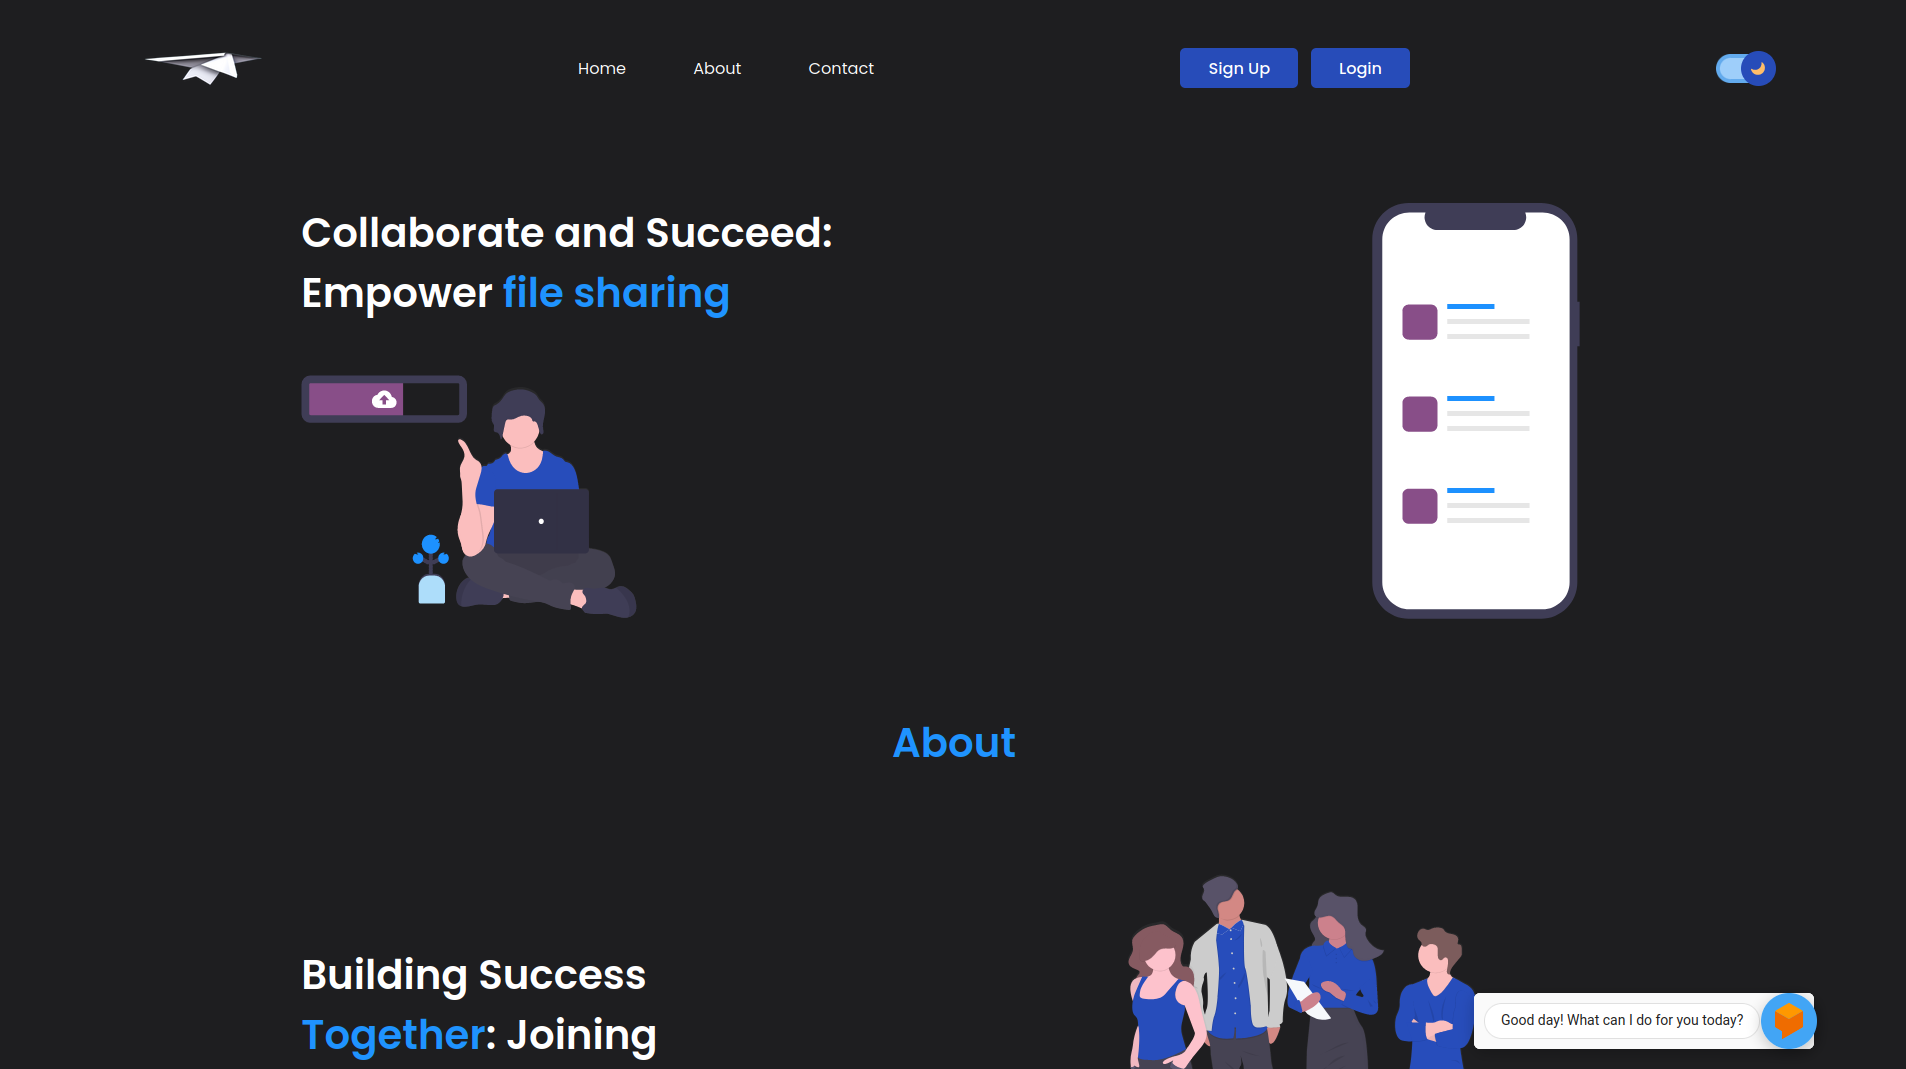
\includegraphics[scale=0.3]{demo/home.png}
    \caption{Home Page}
\end{figure}

"""
    Renders the index page.

    If the user is already authenticated, the function redirects them to the profile page.
    Otherwise, it renders the home.html template with the context indicating whether the user is authenticated.

    Parameters:
    - request: The HTTP request object.

    Returns:
    - If the user is authenticated, a redirect response to the profile page.
    - If the user is not authenticated, a rendered HTML template of the home page.

"""

\begin{figure}[H]
    \centering
    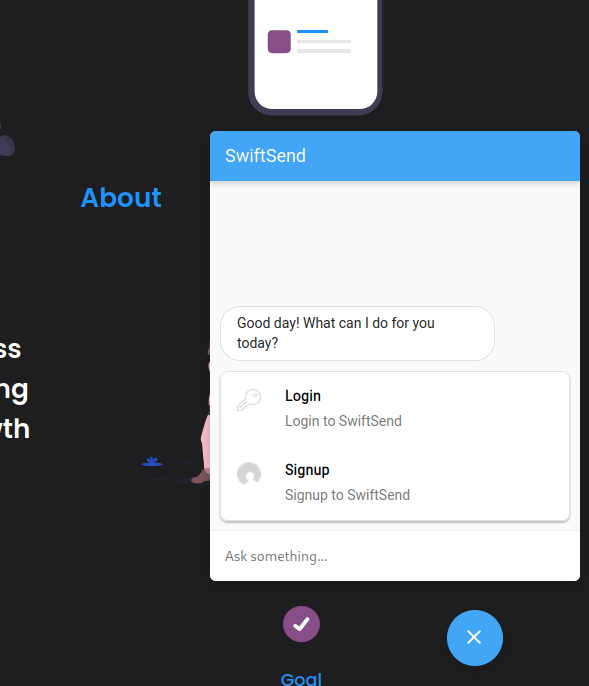
\includegraphics[scale=0.7]{demo/chat.png}
    \caption{Chat bot}
\end{figure}

\subsection{Đăng nhập - Đăng kí}
Trang đăng nhập \\

""" \\
Handles the user login functionality.

If the user is not authenticated, the function processes the login request by validating the CAPTCHA response,
checking the user credentials, and performing necessary actions based on the authentication result.

Parameters:
- request: The HTTP request object.

Returns:
- If the user is not authenticated and the request method is POST, returns a JSON response with messages indicating
  the CAPTCHA validation result, login success, login failure, email activation, or other errors.
- If the user is not authenticated and the request method is GET, renders the login.html template.
- If the user is already authenticated, redirects them to the 'index' page. \\
"""
\begin{figure}[H]
    \centering
    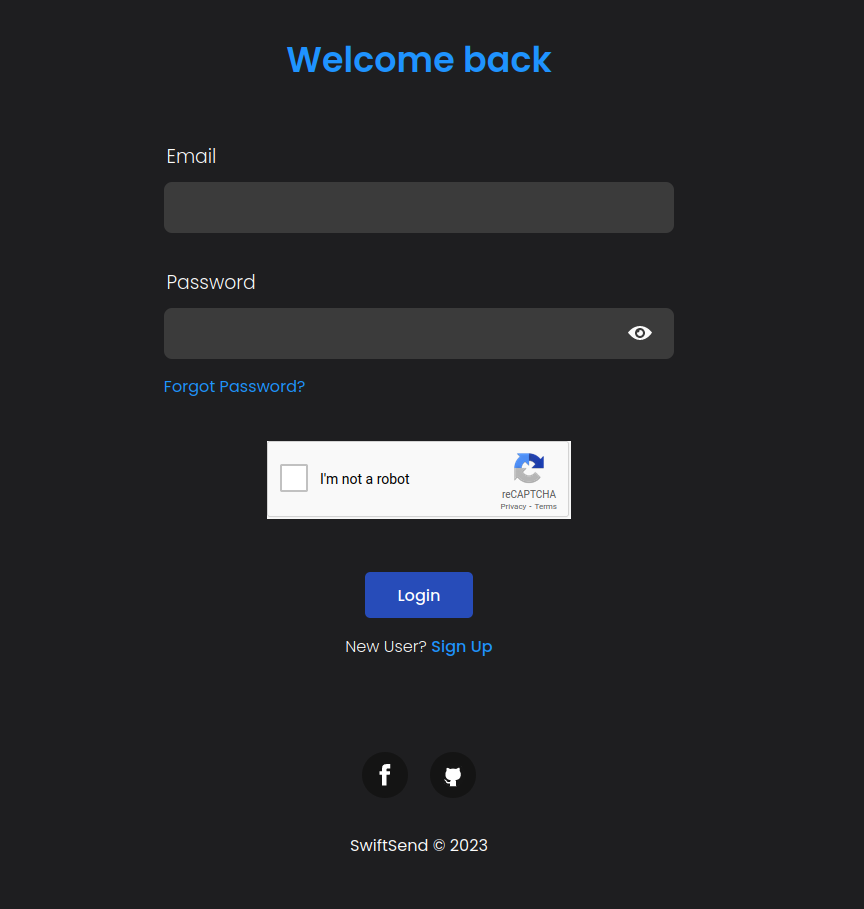
\includegraphics[scale=0.5]{demo/login.png}
    \caption{Trang đăng nhập với captcha}
\end{figure}

Trang đăng kí:

""" \\
Handles the user signup functionality.

If the request method is POST, the function processes the signup request by creating a new user account,
saving the user details, and sending a verification email for account activation.

Parameters:
- request: The HTTP request object.

Returns:
- If the request method is POST and the signup process is successful, redirects to the 'login' page with a success message.
- If the request method is POST and the signup process encounters an error, renders the 'signup.html' template with
  error messages indicating the cause of the failure.
- If the user is already authenticated, redirects to the 'index' page.
- If the request method is GET, renders the 'signup.html' template. \\
"""

\begin{figure}[H]
    \centering
    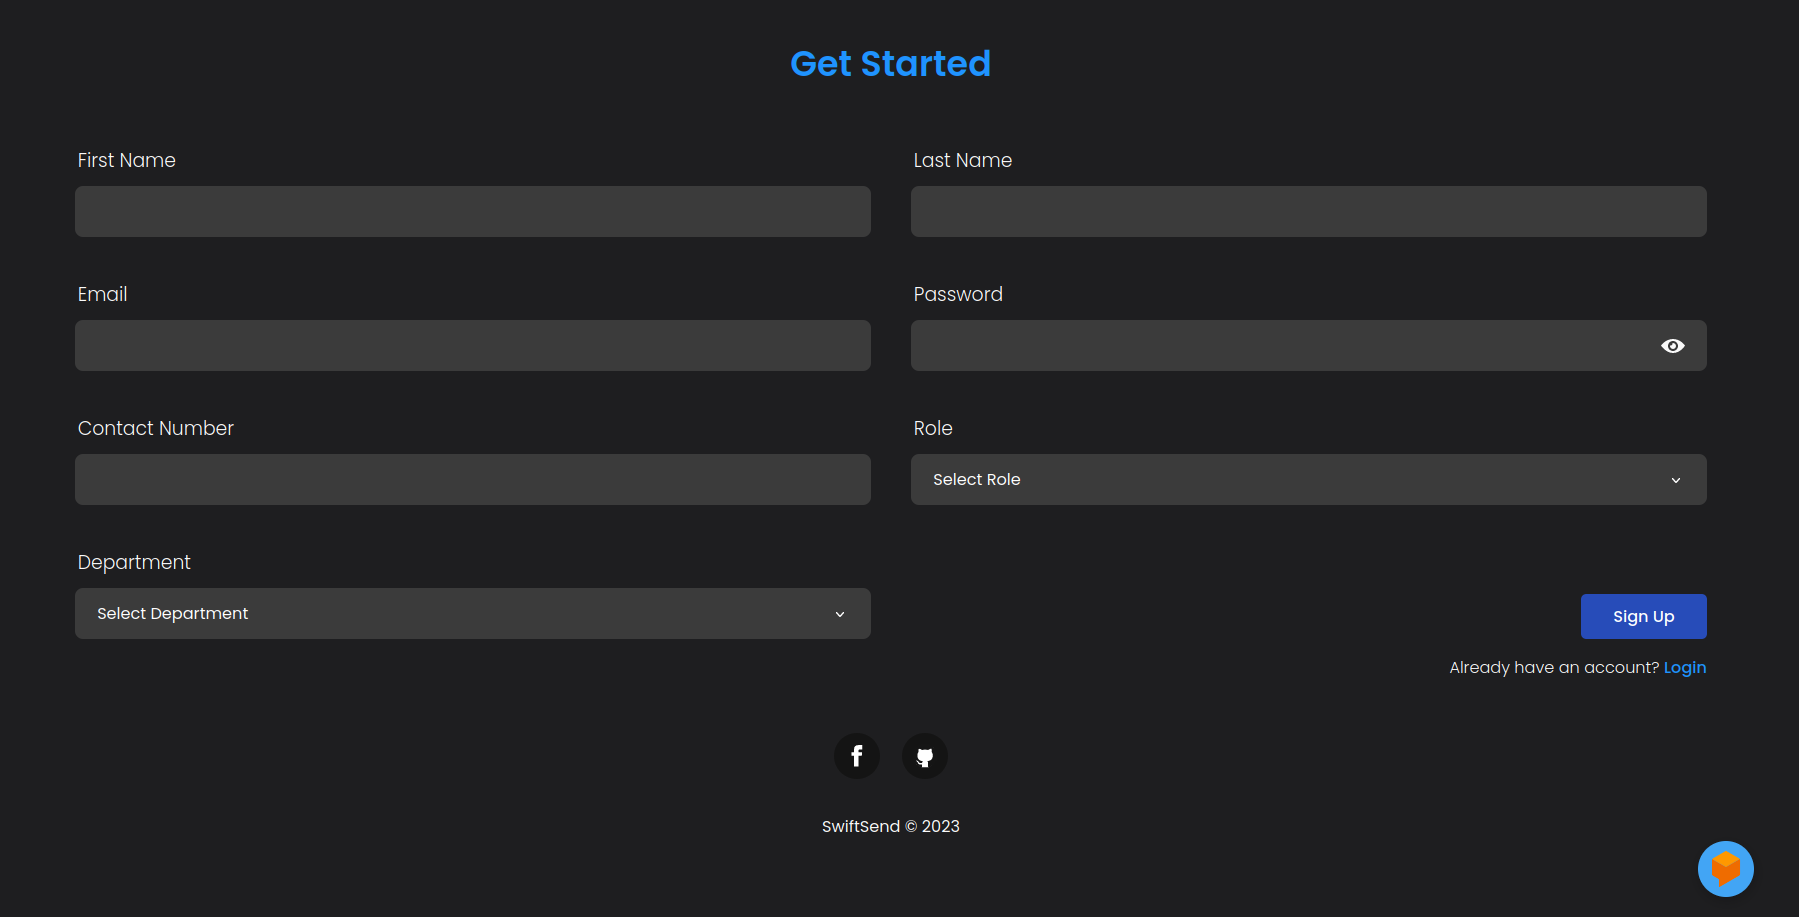
\includegraphics[scale=0.3]{demo/signup.png}
    \caption{Trang đăng kí}
\end{figure}

\subsection{Trang Profile}
\begin{figure}[H]
    \centering
    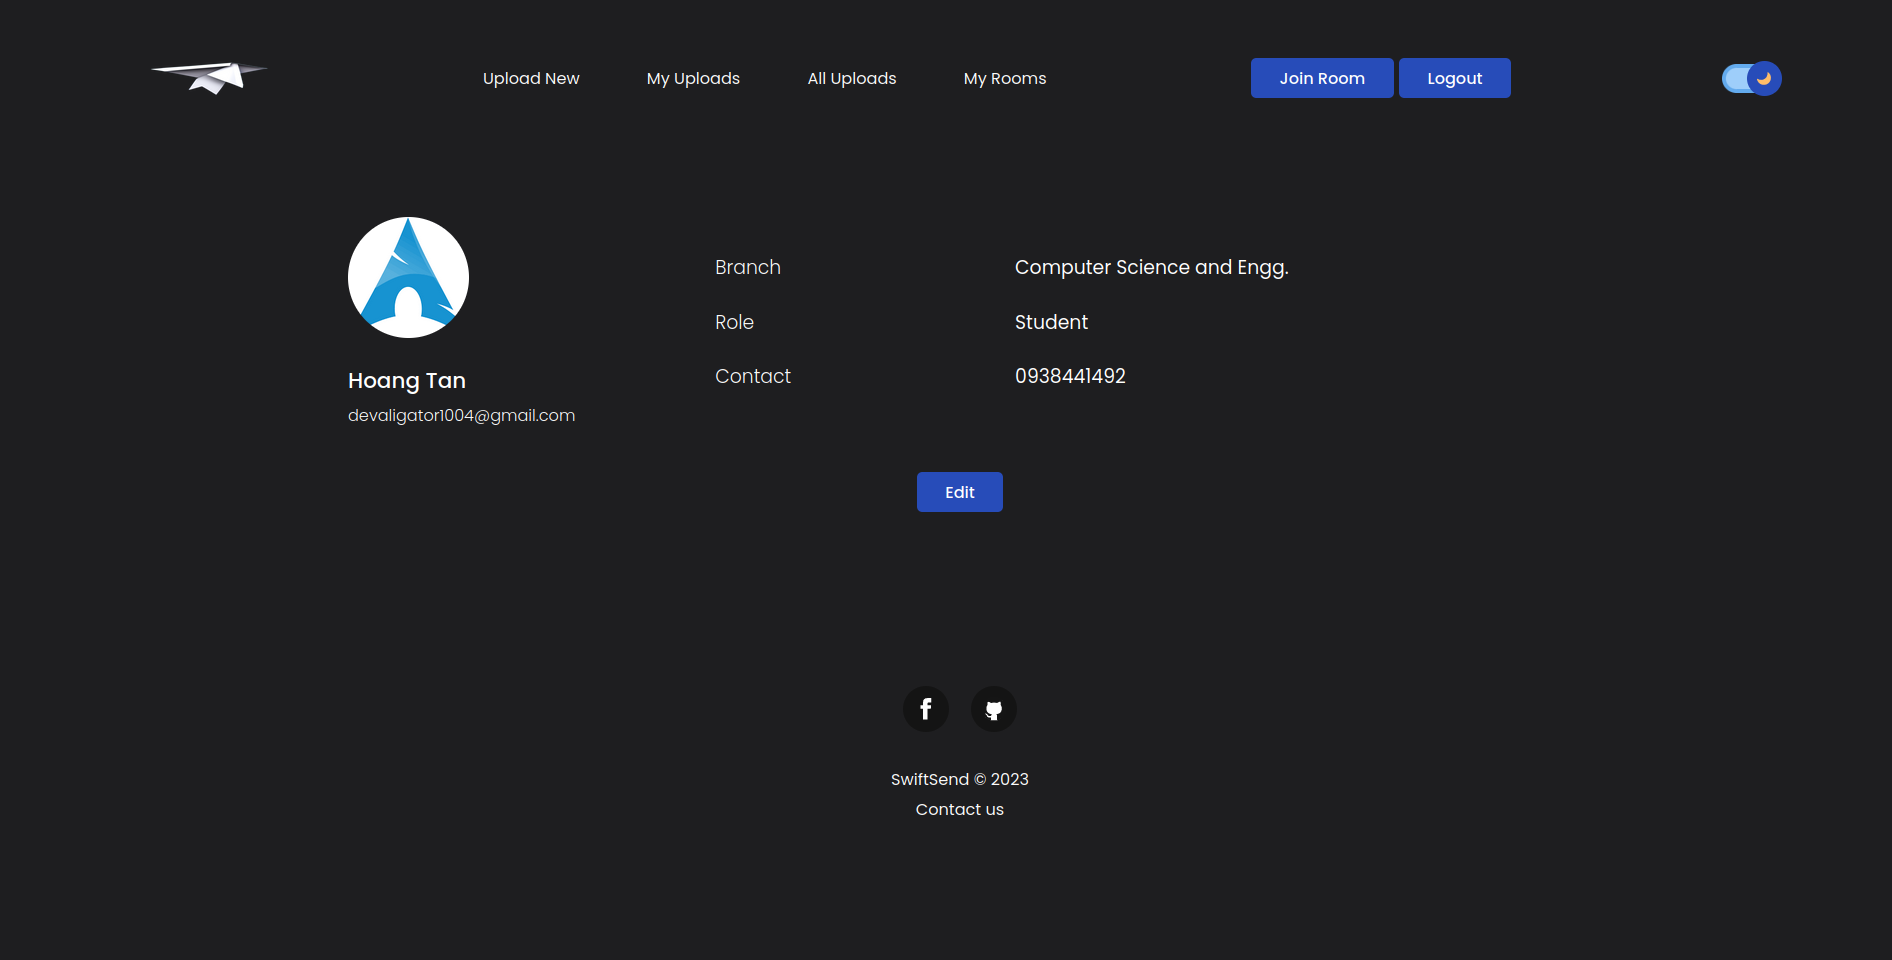
\includegraphics[scale=0.3]{demo/profile.png}
    \caption{Profile}
\end{figure}
""" \\
View function for rendering the user profile page.

Parameters:
- request (HttpRequest): The HTTP request object.

Returns:
- HttpResponse: The response object containing the rendered profile page.

Raises:
- Redirect: If the user is not authenticated, it redirects to the login page.

Notes:
- This function requires the user to be authenticated.
- The user profile page displays information about the logged-in user.
- If the user is a superuser, they have administrative privileges.
- If the user is a staff member, they have staff-specific privileges.
- The 'profile.html' template is used to render the profile page. \\
"""

\subsection{Trang Quản lí các phòng}
\begin{figure}[H]
    \centering
    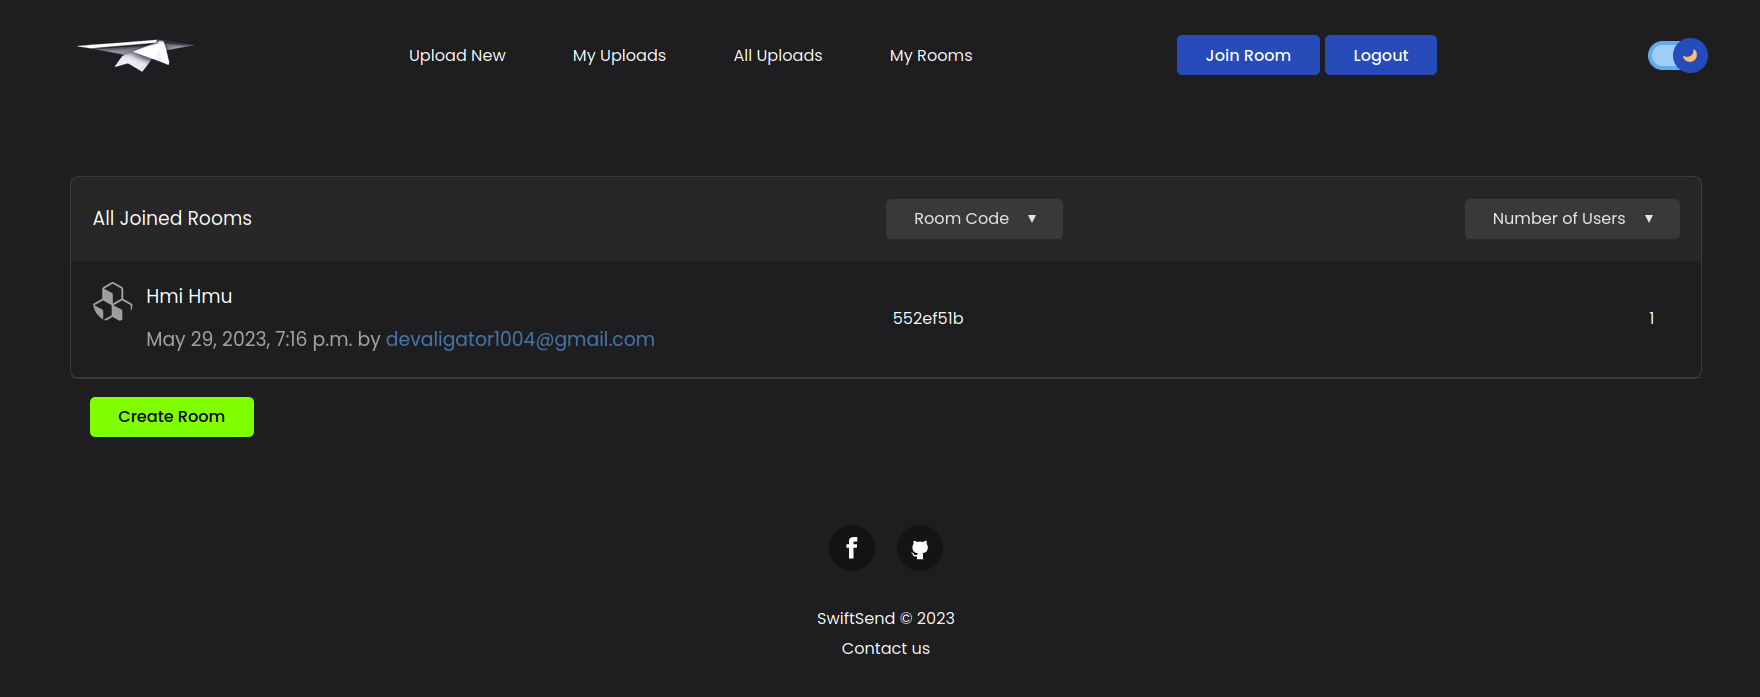
\includegraphics[scale=0.4]{demo/manage_room.png}
    \caption{Quản lí các phòng của user}
\end{figure}

"""
    Renders the user rooms view.

    If the user is not authenticated, the function redirects them to the login page with a message.
    Otherwise, it retrieves the user's signup details and fetches the rooms the user has joined.
    The rooms are then passed as context to the template for rendering.

    Parameters:
    - request: The HTTP request object.

    Returns:
    - If the user is not authenticated, redirects to the 'login' page with an info message.
    - If the user is authenticated, renders the template with the user's joined rooms as context.

    """

\subsection{Tạo và gia nhập phòng}

\begin{figure}[H]
    \centering
    \begin{subfigure}{.5\textwidth}
      \centering
      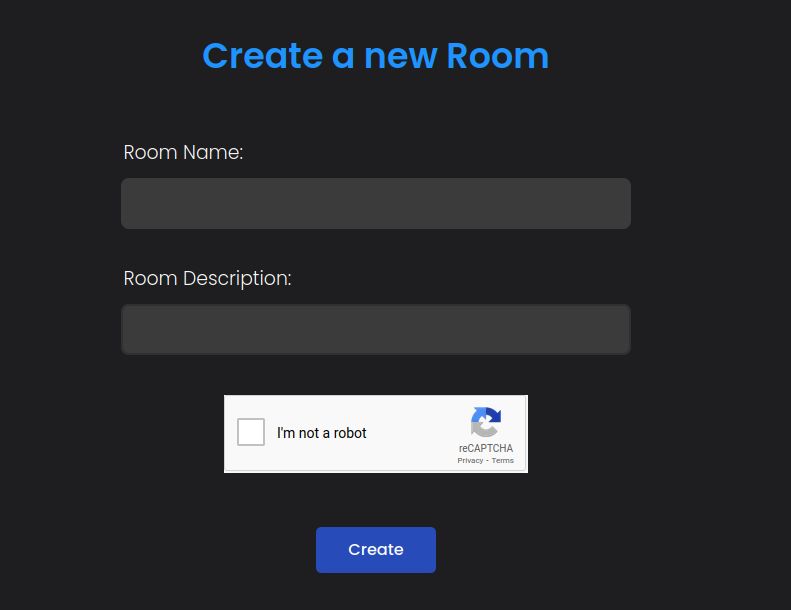
\includegraphics[scale=0.4]{demo/create_room.png}
      \caption{Tạo phòng}
      \label{fig:sub1}
    \end{subfigure}%
    \begin{subfigure}{.5\textwidth}
      \centering
      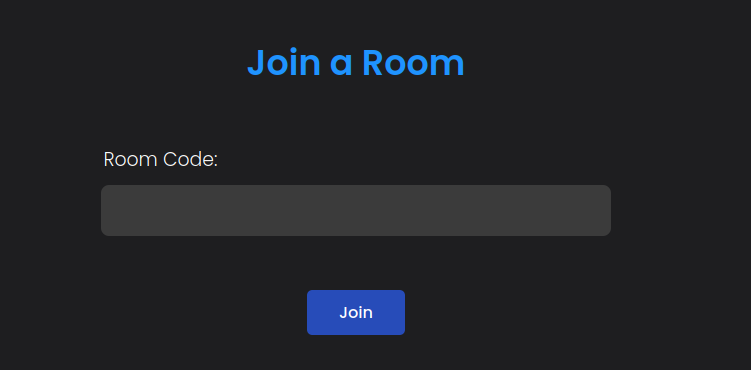
\includegraphics[scale=0.4]{demo/join_room.png}
      \caption{Join Phòng}
      \label{fig:sub2}
    \end{subfigure}
    \caption{Tạo và gia nhập phòng}
    \label{fig:test}
\end{figure}

"""
Handles the creation of a new room.

If the user is not authenticated, the function redirects them to the login page.
If the request method is POST, the function processes the room creation request by extracting the room details,
generating a unique room code, creating a new room instance, associating the creator with the room, and adding the
creator to the joinedrooms field of their signup. It then redirects the user to the viewuserrooms page with a success message.
If the request method is GET, it renders the 'createroom.html' template.

Parameters:
- request: The HTTP request object.

Returns:
- If the user is not authenticated, redirects to the 'login' page.
- If the request method is POST and the room creation is successful, redirects to the 'viewuserrooms' page with a success message.
- If the request method is GET, renders the 'createroom.html' template.

"""

\subsection{Upload file}
    \begin{figure}[H]
        \centering
        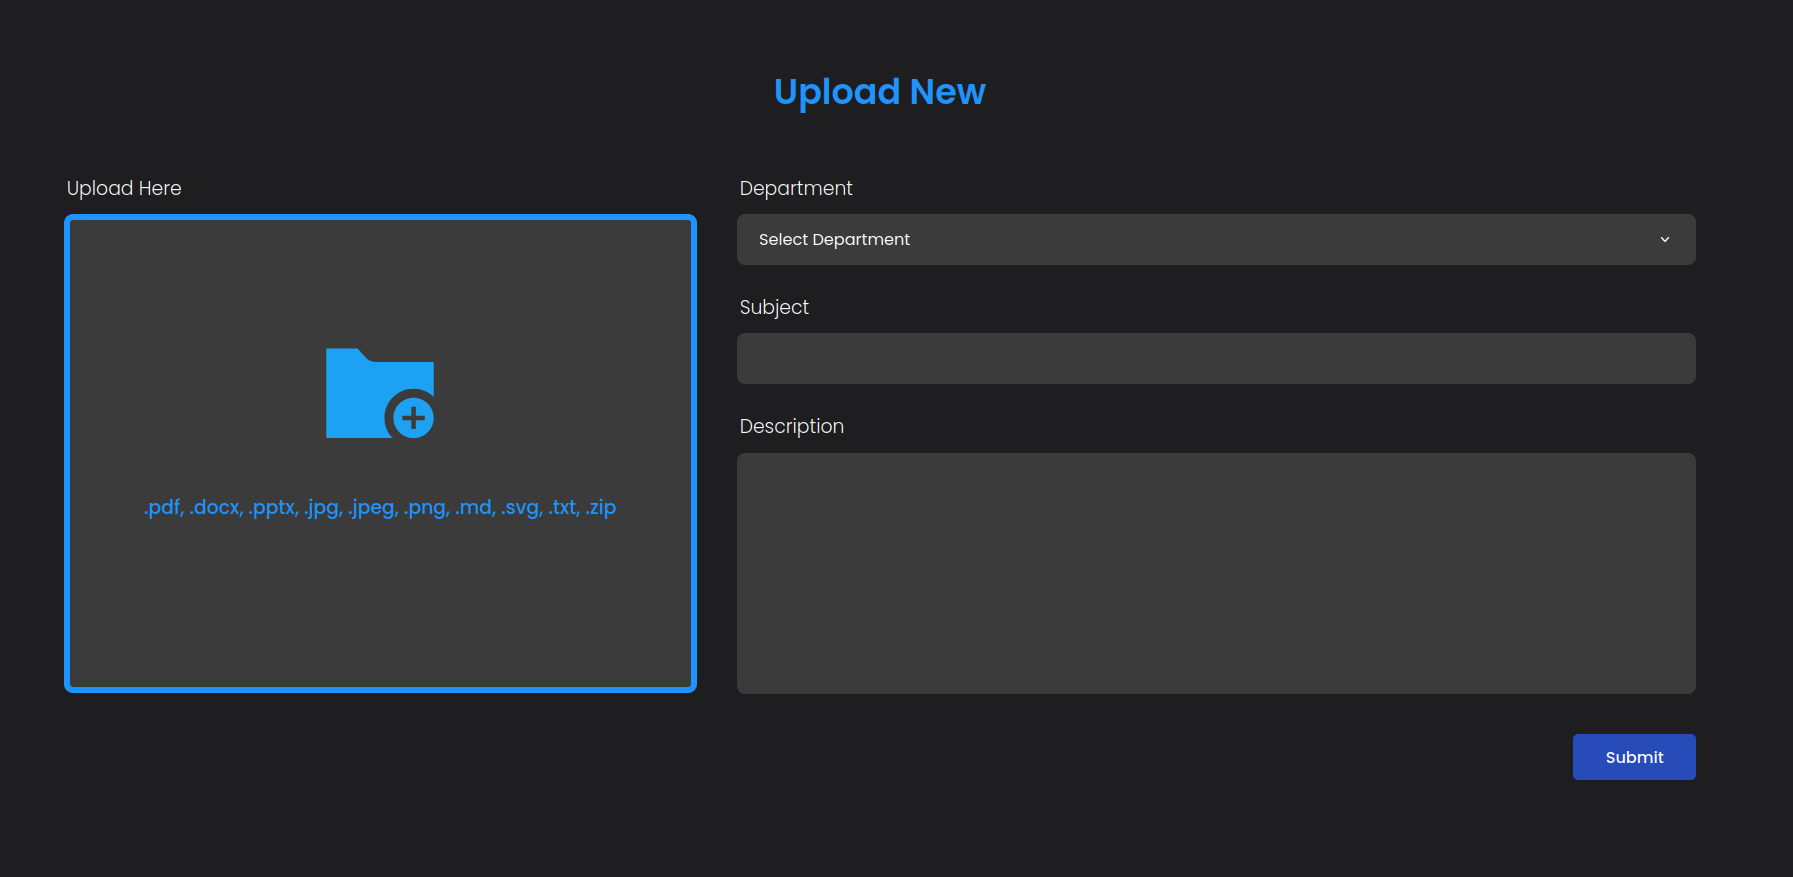
\includegraphics[scale=0.3]{demo/upload.png}
        \caption{Upload new file}
    \end{figure}

    """
    Handles the uploading of notes.

    If the user is not authenticated, the function redirects them to the login page with an info message.
    Otherwise, it retrieves the user's signup details and the rooms they have joined.
    If the request method is POST, the function processes the notes upload request by extracting the note details,
    creating a new Notes instance with the uploaded file, and setting the note status as "Pending".
    It then redirects the user to the 'viewusernotes/open' page with a success message.
    If the note upload encounters an error, it displays an error message.
    If the request method is GET, it renders the 'uploadnotes.html' template with the user's authentication status and
    the rooms they have joined as context.

    Parameters:
    - request: The HTTP request object.

    Returns:
    - If the user is not authenticated, redirects to the 'login' page with an info message.
    - If the request method is POST and the notes upload is successful, redirects to the 'viewusernotes/open' page with a success message.
    - If the request method is GET, renders the 'uploadnotes.html' template with the user's authentication status and joined rooms as context.

    """
\subsection{Xem tất cả các file được upload, và thành viên trong 1 room/department}
\begin{figure}[H]
    \centering
    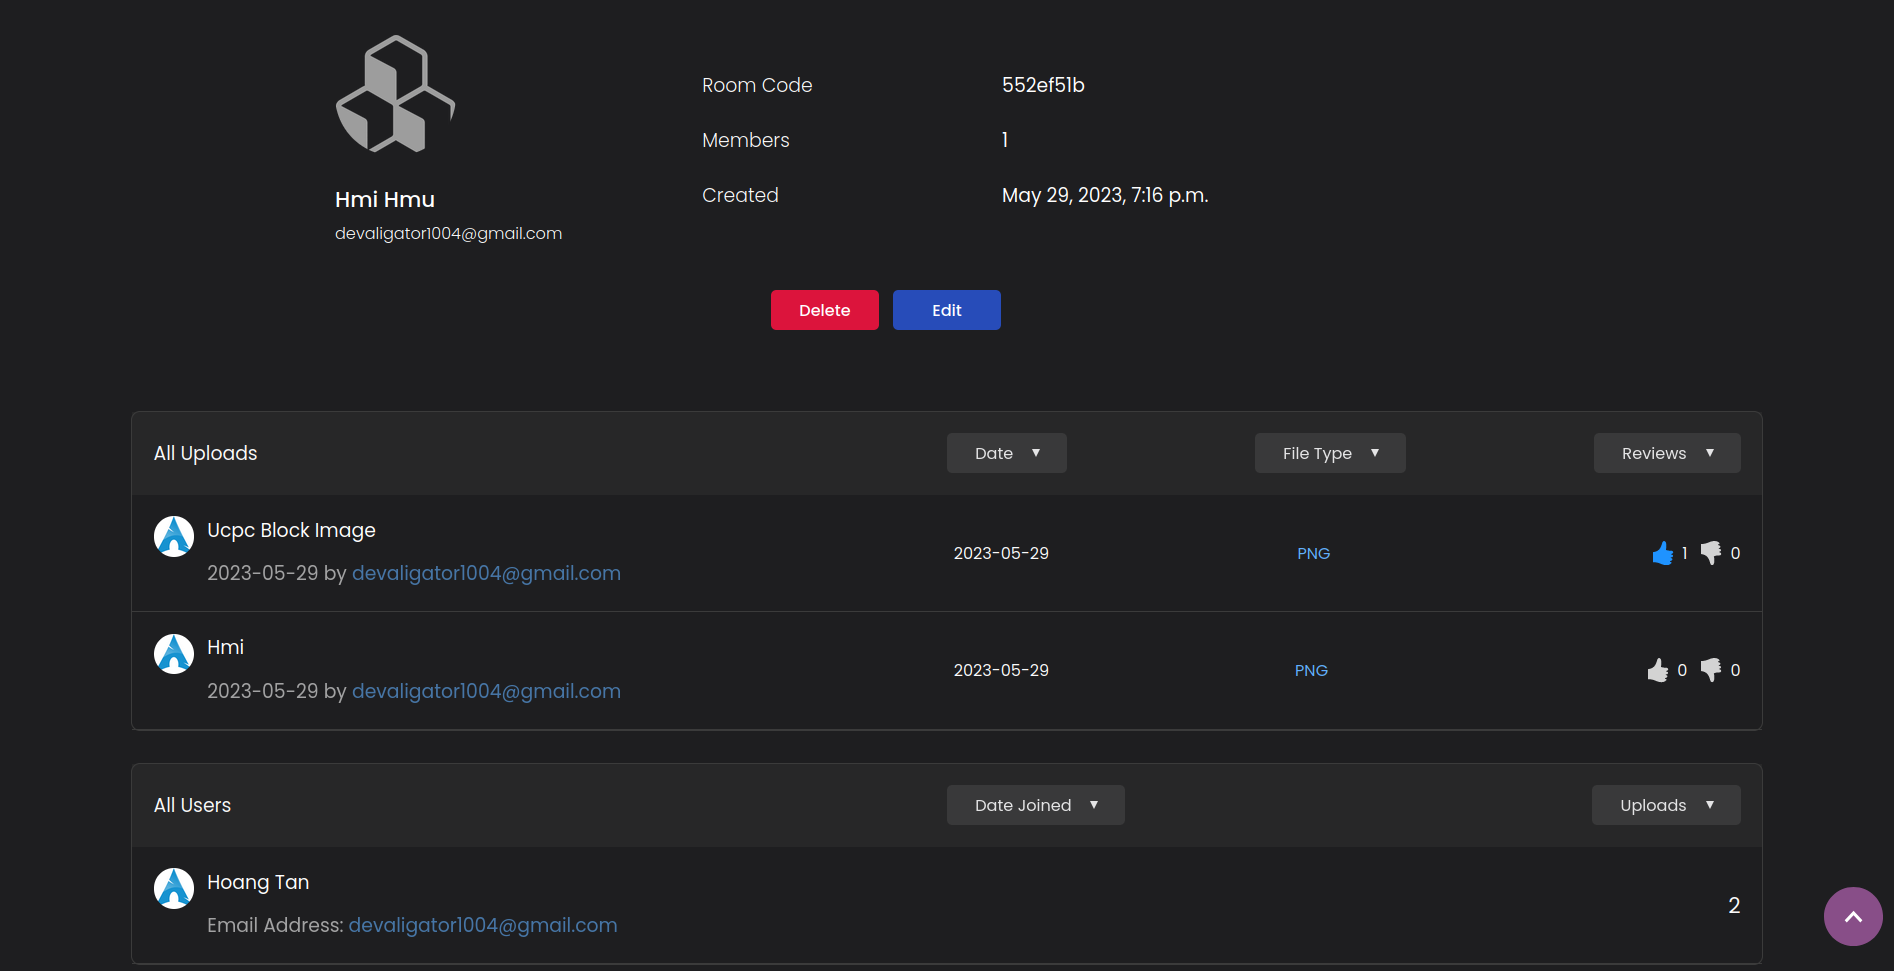
\includegraphics[scale=0.4]{demo/view_room.png}
    \caption{Thông tin phòng}
\end{figure}
"""
    Renders the view for a specific room.

    If the user is not authenticated, the function redirects them to the login page.
    Otherwise, it retrieves the room information based on the provided room code.
    It fetches the members of the room and the notes associated with the room.
    For each note, it retrieves additional details such as the profile photo of the user who uploaded the note,
    whether the current user has liked or disliked the note, and the count of likes and dislikes.
    Additionally, it counts the number of uploads for each member in the room.
    Finally, it renders the 'viewroom.html' template with the room information, notes, and member details as context.

    Parameters:
    - request: The HTTP request object.
    - code: The room code for identifying the room.

    Returns:
    - If the user is not authenticated, redirects to the 'login' page.
    - If the room and associated data are successfully retrieved, renders the 'viewroom.html' template with the room information, notes, and member details as context.

    """

\subsection{Xem các files được tải lên bởi bản thân và mọi người}
\begin{figure}[H]
    \centering
    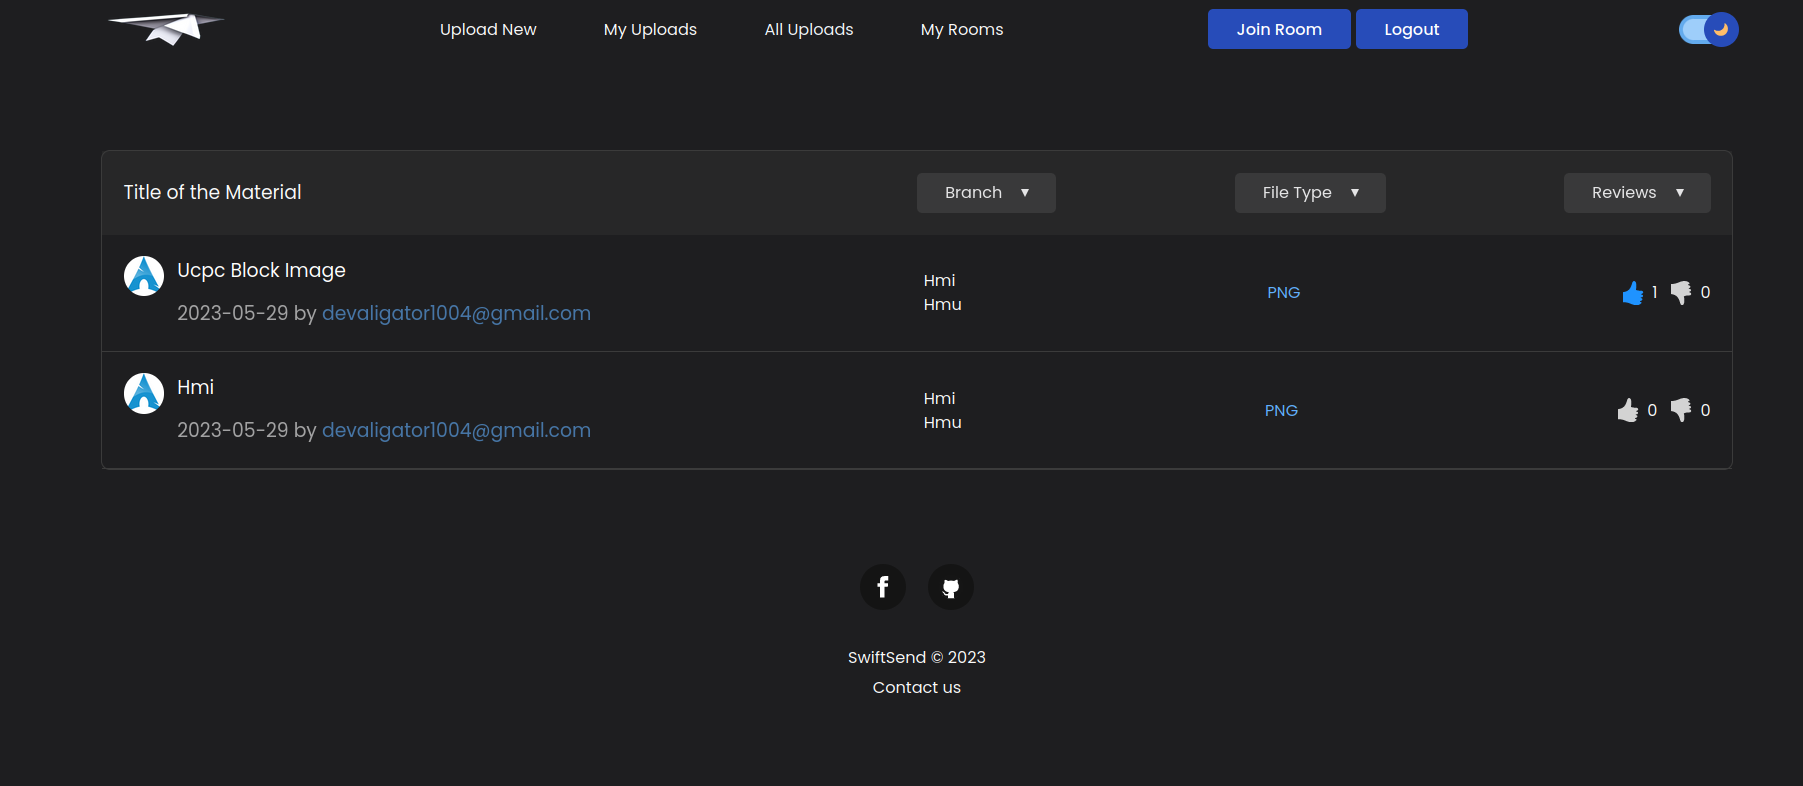
\includegraphics[scale=0.4]{demo/view_uploads.png}
    \caption{Xem tất cả các uploadnotes}
\end{figure}
"""
    Renders the page displaying all accepted user notes.

    If the user is not authenticated, the function redirects them to the login page with an information message.
    Otherwise, it fetches all notes with a status of "Accepted" and performs additional operations to populate
    extra information for each note, such as profile photo, liked/disliked status, and like/dislike counts.
    The function also retrieves the joined rooms for the logged-in user.

    Parameters:
    - request: The HTTP request object.

    Returns:
    - If the user is not authenticated, redirects to the 'login' page with an information message.
    - If the user is authenticated, renders the 'viewallusernotes.html' template with the following context data:
        - 'notes': A queryset of all accepted notes.
        - 'viewall': A boolean value indicating that all notes are being viewed.
        - 'reviewed': A boolean value indicating that the notes have been reviewed.
        - 'rooms': A queryset of joined rooms for the logged-in user.
    """

\subsection{Tải file}
\begin{figure}[H]
    \centering
    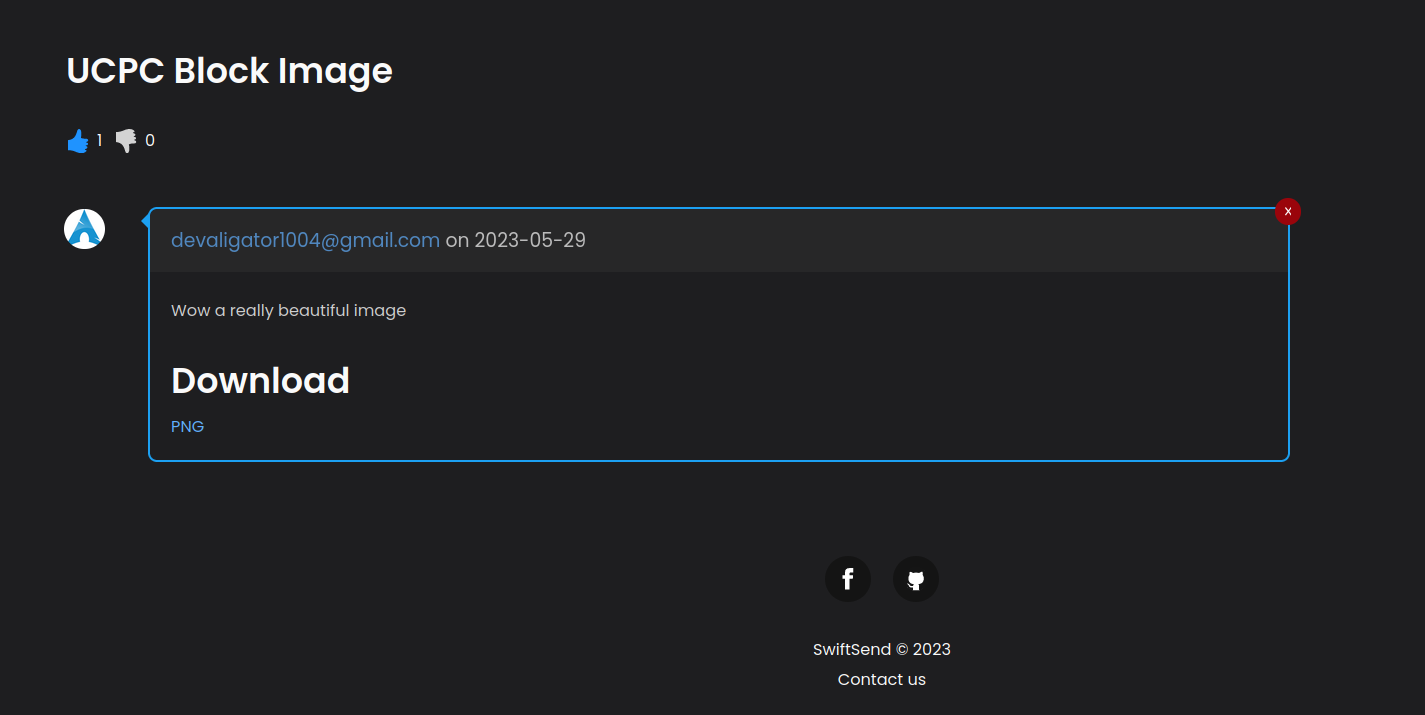
\includegraphics[scale=0.5]{demo/download.png}
    \caption{Giao diện tải file được chọn}
\end{figure}

"""
Renders the view for a specific note.

If the user is not authenticated, the function redirects them to the login page.
Otherwise, it attempts to retrieve the note based on the provided ID.
It fetches additional details for the note, such as the profile photo of the user who uploaded the note,
whether the current user has liked or disliked the note, the count of likes and dislikes,
and whether the current user owns the note.
Finally, it renders the 'viewnote.html' template with the note details as context.

Parameters:
- request: The HTTP request object.
- id: The ID of the note for identifying the note.

Returns:
- If the user is not authenticated, redirects to the 'login' page.
- If the note is successfully retrieved and additional details are fetched, renders the 'viewnote.html' template with the note details as context.
- If the note is not found, returns an HttpResponse indicating that the resource is not available.

"""

\subsection{Đăng nhập với Google}
\begin{figure}[H]
    \centering
    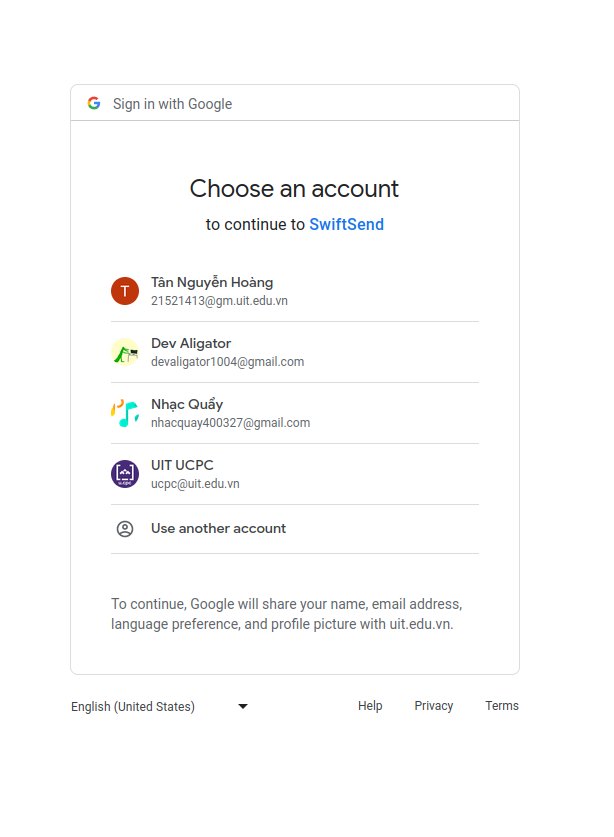
\includegraphics[scale=0.5]{demo/google.png}
    \caption{Đăng nhập với google}
\end{figure}
"""
    Custom adapter for the user account in the application.

    Inherits from the DefaultAccountAdapter class and provides custom methods for saving a user,
    creating a new user, and linking a social account to a local user account. \\


    Overrides the default saveuser() method to save additional user details from the registration form.

        Parameters:
        - request: The HTTP request object.
        - user: The user instance.
        - form: The registration form instance.
        - commit: Boolean value indicating whether to save the user object immediately.

        Returns:
        - The saved user object. \\


        Overrides the default newuser() method to set the user as active by default.

        Parameters:
        - request: The HTTP request object.

        Returns:
        - The newly created user object.
"""

\subsection{Staff - Xem thông tin các Users}
\begin{figure}[H]
    \centering
    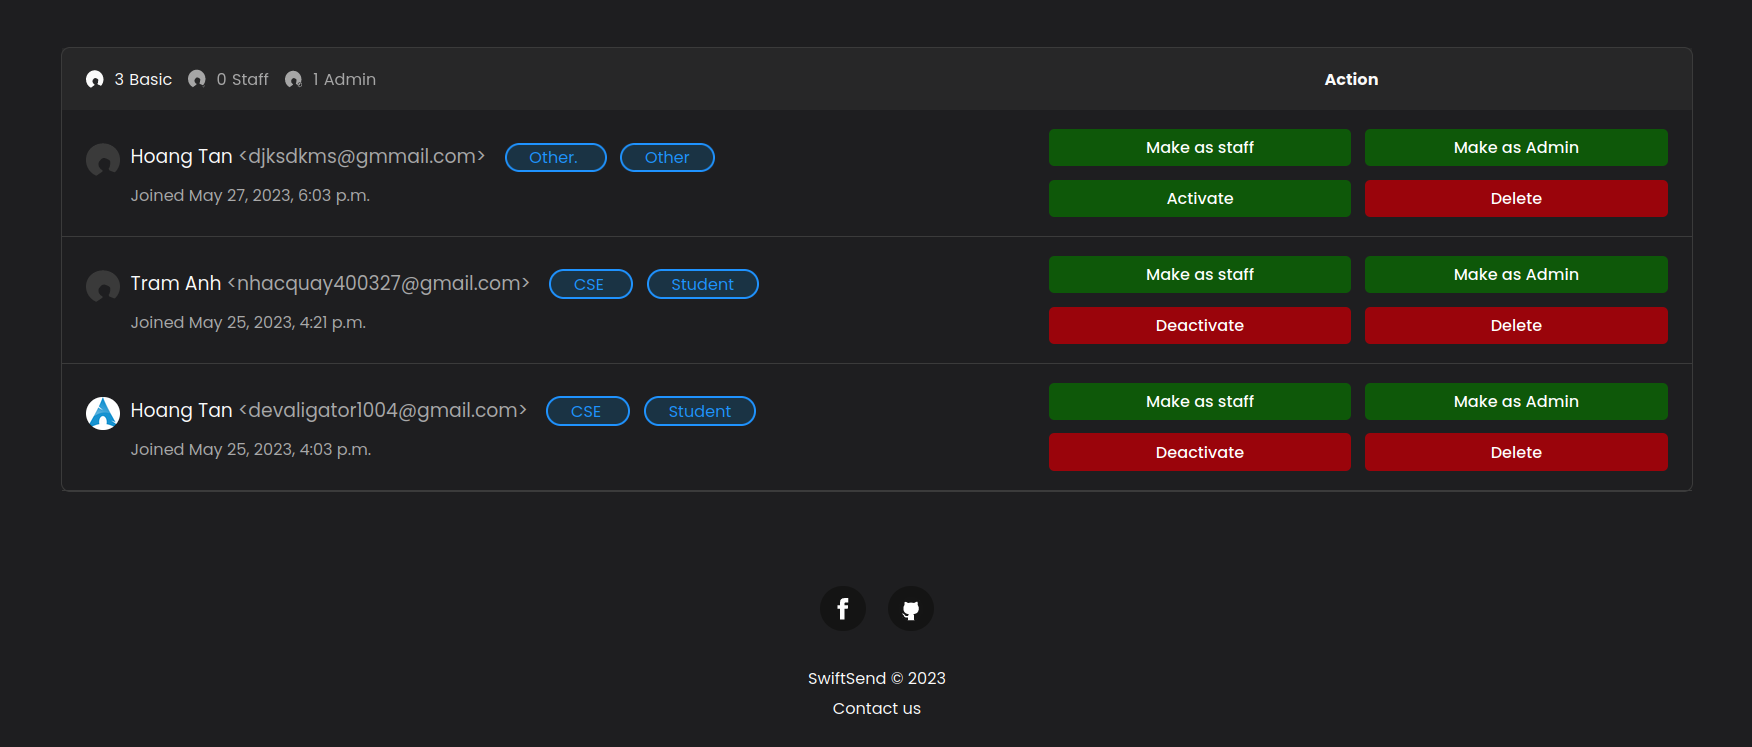
\includegraphics[scale=0.4]{demo/view_users.png}
    \caption{Quản lí tất cả users}
\end{figure}

"""
    View function for the superadmin dashboard in the UCPC application.

    Displays users based on the specified type (basic, staff, admin) for superadmin users.

    Parameters:
    - request: The HTTP request object.
    - type: The type of users to display ("basic", "staff", "admin").

    Returns:
    - The rendered HTML template with the users and additional context variables.
    """

\subsection{Staff - Review Note}
\begin{figure}[H]
    \centering
    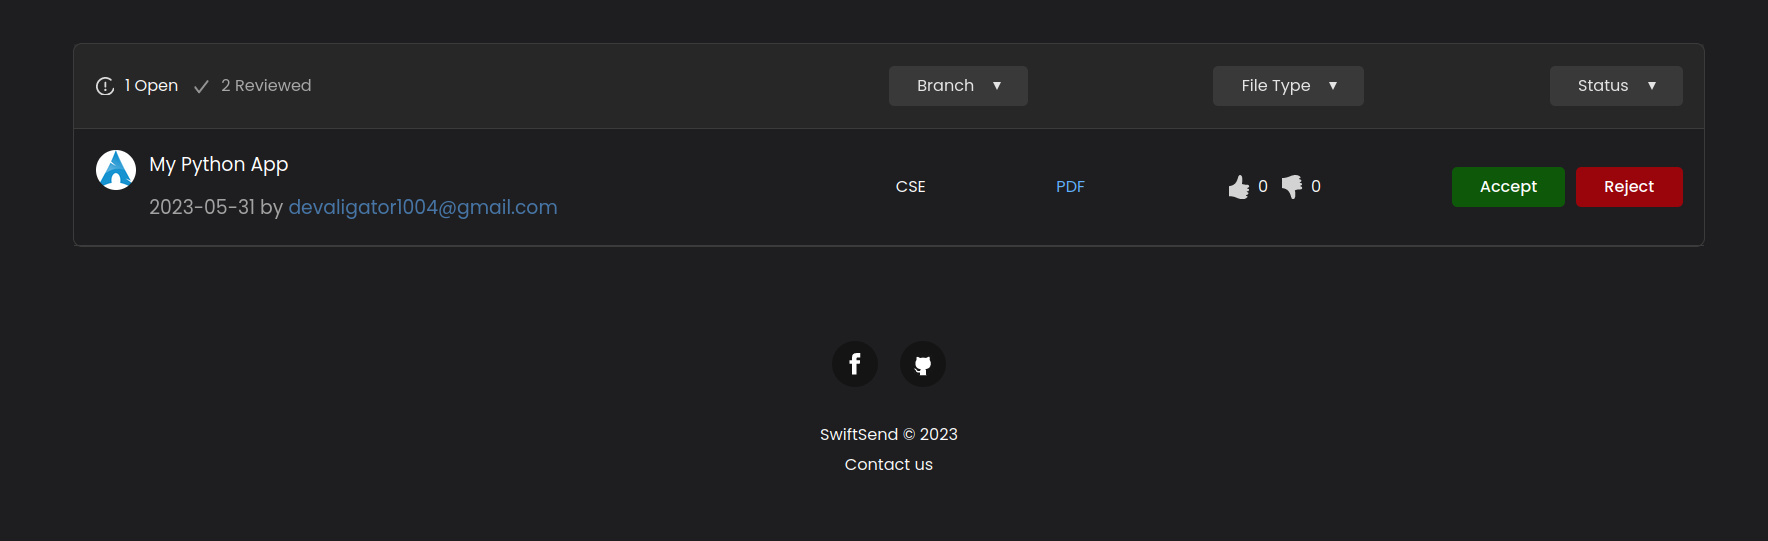
\includegraphics[scale=0.4]{demo/review.png}
    \caption{Review note}
\end{figure}

"""
View function for the admin dashboard in the UCPC application.

Displays the notes based on the specified type (reviewed or pending) for admin users.

Parameters:
- request: The HTTP request object.
- type: The type of notes to display ("reviewed" or "pending").

Returns:
- The rendered HTML template with the notes and additional context variables.
"""
\section{Đôi lời cuối}
Mình muốn nhấn mạnh rằng những gì demo phía trên chỉ là một phần tính năng mà ứng dụng này cung cấp. Ngoài những gì đã được trình bày, App còn rất nhiều tính năng khác như chỉnh sửa hồ sơ cá nhân, chỉnh sửa phòng, tạo mã QR, tích hợp lưu trữ đám mây, gửi email kích hoạt và nhiều tính năng nhỏ khác.

Để khám phá đầy đủ và chi tiết ứng dụng, mình khuyến khích trải nghiệm trực tiếp tại \href{https://aligator.pythonanywhere.com}{website} hoặc truy cập vào \href{https://github.com/Dev-Aligator/SwiftSend-Web}{GitHub} để xem source code cùng docstring chi tiết. 

Trong trường hợp bạn muốn tìm xem những demo cùng docstring chi tiết của ứng dụng, vui lòng ghé qua trang wiki của SwiftSend, mình sẽ cố gắng cập nhật sớm nhất có thể.


\end{document}
